
\section{Redundancy-based Cache Oblivious Data Layout Algorithm}

\subsection{Definitions}

Let us assume that the walkthrough scene data, including all the levels of details of the model, are partitioned into equal sized data blocks (say 4KB) called data units. This is the atomic unit of data that is accessed and fetched from the disk. Typically, vertices and triangles that are spatially together (and belong to the same level of detail), have high chances of being rendered together, and hence can be grouped together in a data unit. All the data units required to render a scene from a viewpoint is labeled as an {\em access requirement}. In order to minimize the number of access requirements, the navigation space in the walkthrough scene, which defines the space of all possible view points, is partitioned into grids and all the viewpoints within each grid is grouped together to define one access requirement. Thus the number of grid partitions define the number of access requirements. Primitives in a data unit can be visible from many viewpoints, and hence that data unit will be part of many access requirements. \\
\\
That was one example of data units and their access requirements. In general, the access requirements are determined by the application and are meant to be sets of data units that are likely to be accessed together. \\
\\
Given a linear ordering of data units that may eventually be the order in which they are stored in the hard drive, for an access requirement $A$, the total span of $A$ is the total number of data units between the first and last data units that use $A$. If a data unit is not required by $A$ but lies between the first and last unit of $A$ then it is still counted in the span of $A$. Figure \ref{singleAR} shows a linear order of data units and three different access requirements shown by solid, double-dashed and dotted lines. The span of an access requirement is the number of blocks between the first and the last data unit that use that access requirement. For example, for the access requirement shown with the solid line, the span is 11; the double-dashed line one has span 12, and the dotted line one has span 11. A data unit can be part of many access requirements. In the example shown in Figure 1, data units 1, 4 and 12 are part of two access requirements and data unit 9 is part of all three. \\
\\
\begin{figure}[ht]
\centering
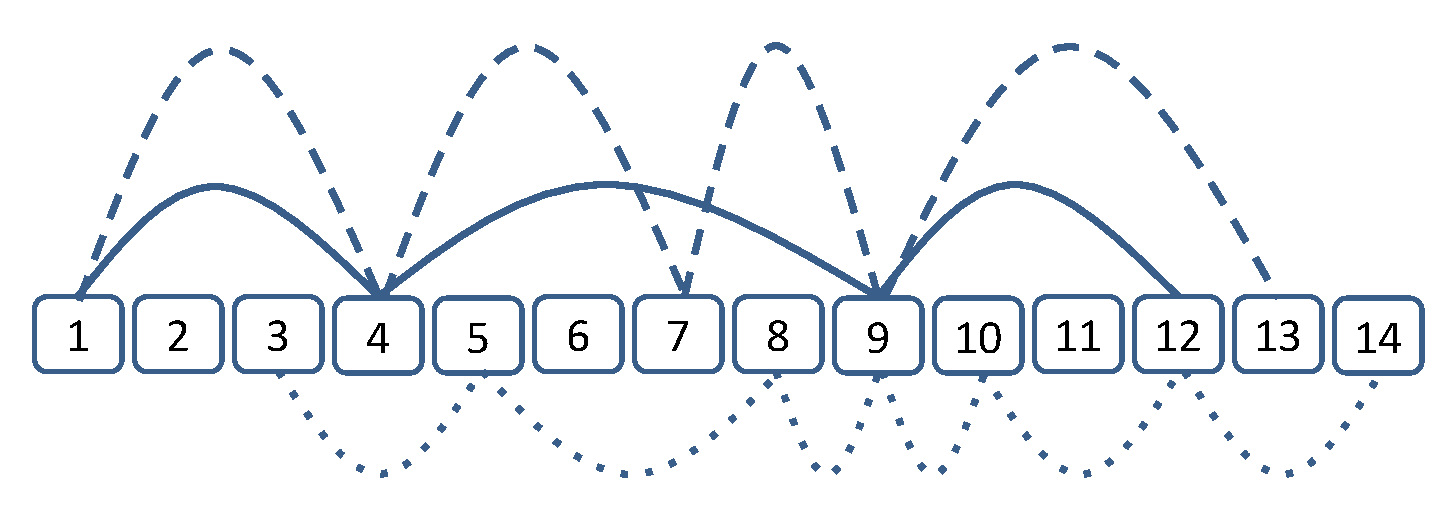
\includegraphics[width=\columnwidth]{AccessReqsFigure.pdf}
\caption{Illustration of linear order of data units and three example access requirements.
The lines connect data blocks that belong to the same access requirement
and represent parts of the span of an access requirement.}
\label{singleAR}
\end{figure}

\subsection{Seek Time Measure}
Given a linear order of data units and the access requirements, and assuming that each access requirement
is equally likely to be used, we would like to estimate the seek time for that application.
For each access requirement the read head of the hard disk has to move from the first data block to the last
irrespective of whether the intermediate blocks are read or skipped. Hence the span of an access requirement
is a measure of seek time - time taken to seek the last data unit starting from the first data unit.
Let $I$ be the set of access requirements and $A_i$ represent the span of the access requirement $i$.
Then estimated total seek time EST is given by 
\[
EST = \sum_{i \in I}{A_i}
\]
It is interesting to note that \cite{cacheobliviouslayout}
used span to measure the expected number of cache misses.
Typically, with every cache miss, the missing data will be sought in the disk and fetched,
thus adding to the seek time. Hence using span to measure the seek time is justified.


\subsection{Algorithm Overview}

In \cite{cacheobliviouslayout}, the only allowed operation on the data units is
the move operation and the optimal solution is computed using only that
operation. For our purposes, we are allowed to copy data units, move them, and
delete them if they are not used. Using these operations, our goal is to minimize EST
while keeping the number of redundant copies as low as possible. After constructing a cache oblivious layout 
of the data set to get an initial ordering of data units, we copy one data unit to another location, and reassign 
one or more of the access requirements that uses the old copy of the data unit to the new copy, such that the EST is reduced. 
If all the access requirements that used the old copy, now use the new copy of the data unit, then the old copy is deleted. 
We repeat this copying and possible deletion of individual data units until our redundancy limit has been reached. \\
\\
{\bf Blocks to Copy:} Note that the span of an access requirement does not
change by moving an interior data unit to another interior location. Cost can
be reduced only by moving the data units that are at the either ends of the access
requirement. This observation greatly reduces the search space of data units to
consider for copying. Additionally, for the sake of simplicity of the algorithm, we operate
on only one data block at a time. \\
\\
{\bf Location to Copy:} Based on the above observation, given an access requirement, we can possibly move the beginning or the end data units of an access requirement to its interior. This will reduce its span, thus reducing the EST for the layout. However, if the new location of the data unit is in the span of other access requirements, such as location 11 in Figure \ref{singleAR}, it increases the span of those accesses by one unit. Let $j$ be the new location for the start or end data unit of an access requirement $i$. Let $\Delta A_i$ denote the change in the span of the access requirement $i$ by performing this copying operation. With the access requirements whose span overlaps $j$, their span would be increased by one. Let  $k_j$ denote the number of access requirements whose span overlaps at location $j$.  The reduction in EST by performing this copying operation is given by 
\[ 
\Delta EST_C(i,j) = \Delta A_i - k_j 
\]
where $C$ denotes {\it copying} the data unit for access requirement $i$ to the location $j$. We find the location $j$ that is 
\[
argmax_j(\Delta EST_C(i,j))
\]
which signifies where the start or end data unit of the access requirement $i$ needs to be copied, using a simple linear search through the span of $i$. \\
\\
{\bf Assignment of Copies to Access Requirements:} The above operation would result in two copies of the same data unit, say $d_{old}$ and $d_{new}$. Clearly the new copy $d_{new}$ in location $j$ will be used by the access requirement $i$.  But $d_{old}$ could be accessed by
multiple access requirements. All other access requirements that accesses $d_{old}$ can either continue to use $d_{old}$ or use $d_{new}$ depending on the overall effect on their span. Let $S$ be the set of access requirements whose span does not increase by using $d_{new}$ instead of $d_{old}$. Now the total benefit by copying the data unit $d_{old}$ of the access requirement $i$ to the new location $j$ is
\begin{equation}
\Delta EST_C(i,j) = \Delta A_i - k_j + \sum_{s\in S}\Delta{A_s}.
\label{eq:copyingcost}
\end{equation}
\\
{\bf Moving versus Copying:} Let $T$ be the set of access requirements whose span will increase by accessing $d_{new}$ instead of $d_{old}$. Further, let $k_{old}$ be the number of access requirements in whose span $d_{old}$ is. If we force all the access requirements that uses $d_{old}$ to use $d_{new}$ and then delete $d_{old}$ -- in other words, if we move $d$ instead of copying -- then the benefit of this move would be given by
\[
 \Delta EST_M(i,j) = \Delta A_i - k_j + \sum_{s\in S}\Delta{A_s} + \sum_{t\in T}\Delta{A_t} + k_{old}
\]
\[
 \Delta EST_M(i,j) = \Delta EST_C(i,j) + \sum_{t\in T}\Delta{A_t} + k_{old}
\]
where $\Delta EST_M(i,j)$ gives the benefit of {\it moving} a start or end data unit of the access requirement $i$ to position $j$. Note that each of $\Delta A_t$ is negative. Hence the benefit of moving might be more or less than the benefit of copying depending on the relative values of $\sum_{t\in T}\Delta{A_t}$ and $k_{old}$. But the main advantage of moving instead of copying is that this operation does not increase the redundancy thus it keeps the storage requirement the same. So we perform moving instead of copying as long as $\Delta EST_M(i,j)$ is positive.\\
\\
{\bf Data Unit processing order:} We now need to figure out how to use this
information to decide in what order the copying and moving should be done. We will make two heaps: $E_M$ and $E_C$. The $E_M$ heap will organize the move operations and consist of the values of $\Delta EST_M(i,j)$ for the start and end data units for all access requirements $i$ where the units are put in their optimal location $j$. The $E_C$ heap will be the same thing except it will organize the copy operations and consist of the values of $\Delta EST_C(i,j)$.\\
\\
You empty the $E_M$ heap first as long as the top of the heap is positive. After each removal and processing, you update $\Delta EST_M$ and $\Delta EST_C$ of the affected access requirements and update the corresponding heaps. If there are no more data units where $\Delta EST_M$ is positive, then process the top of $E_C$. After processing a copied data unit from the top of heap $E_C$, the heaps $E_C$ and $E_M$ are again updated with new values for the affected access requirements. If this introduces an element in the top of $E_M$ heap with positive values, the $E_M$ heap is processed again. This process gets repeated until we run out of space for more redundant data units. As a summary, the psuedo-code of this algorithm is shown as algorithm \ref{pseudocode}.

\begin{algorithm}
Input: Data units and their access requirements (AR) \;
\For{start and end unit of each AR i}{
	Find optimal location $j$ for copy\;
	Calculate $\Delta EST_M(i,j)$ and insert into $E_M$ \;
	Calculate $\Delta EST_C(i,j)$ and insert into $E_C$ \;
}
\While{{\bf true}}{
		\While{top element of $E_M$ is positive}{
			Pop top element and move the data unit to its destination \;
			Update $E_M$ and $E_C$ \;
		}
		\eIf{there is more space for redundancy}{
		Pop top element and copy the data unit to its destination \;
		Update $E_M$ and $E_C$ \;
		}{{\bf break}}
}
\caption{Pseudo-code for our algorithm}
\label{pseudocode}
\end{algorithm}

